\chapter{Diagramas de flujo de los comandos}
\label{diagramasFlujo}
\begin{figure}[H]
    \begin{center}
        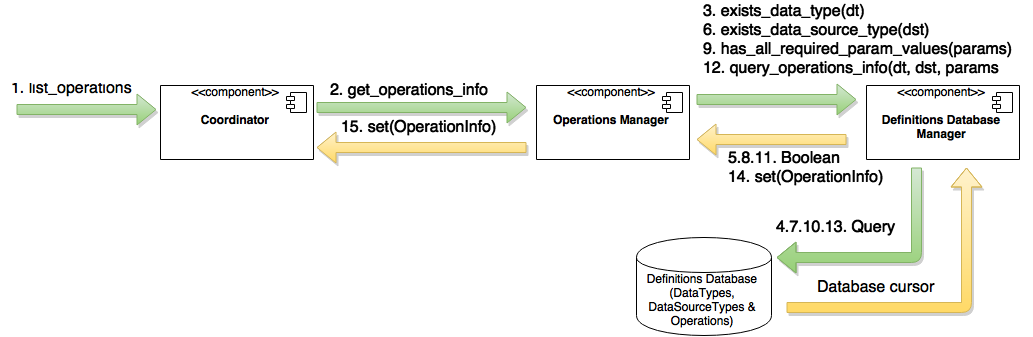
\includegraphics[width=0.95\textwidth]{figures/list_operations}
        \caption{Flujo de ejecución del comando \texttt{list}}
    \end{center}
\end{figure}

\begin{figure}[H]
    \begin{center}
        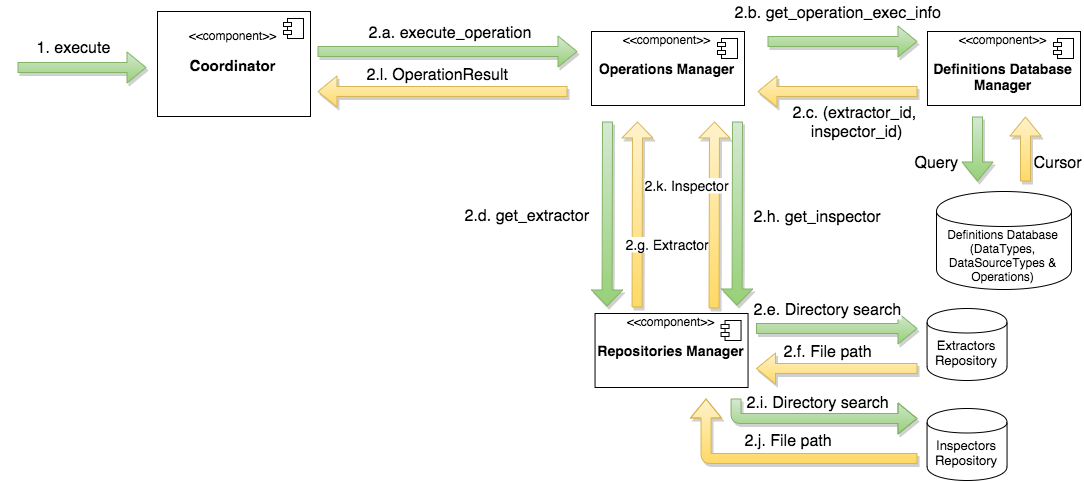
\includegraphics[width=\textwidth]{figures/execute_operations}
        \caption{Flujo de ejecución del comando \texttt{execute}}
    \end{center}
\end{figure}

\begin{figure}[H]
    \begin{center}
        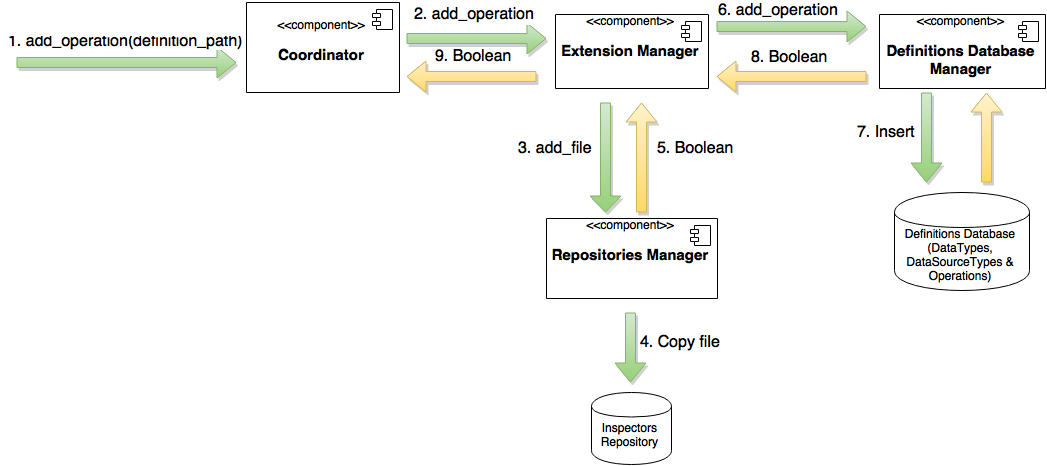
\includegraphics[width=\textwidth]{figures/add_operation}
        \caption{Flujo de ejecución del comando \texttt{add\_operation}}
    \end{center}
\end{figure}

\begin{figure}[H]
    \begin{center}
        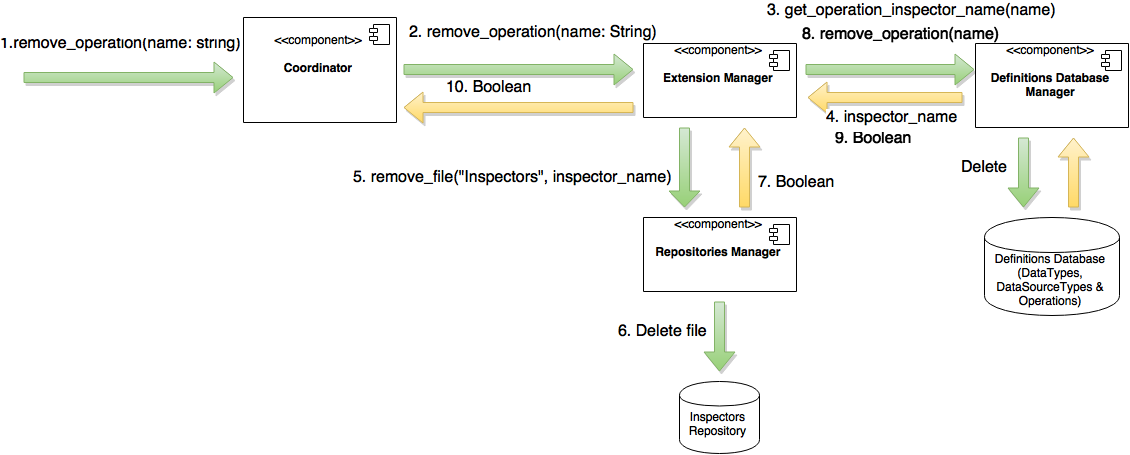
\includegraphics[width=\textwidth]{figures/remove_operation}
        \caption{Flujo de ejecución del comando \texttt{remove\_operation}}
    \end{center}
\end{figure}
